One of the main objectives of \sys run-time is to restrict tasks to interface only with the volatile memory, since volatile memory access is relatively cheaper than non-volatile memory access, as we already have shown experimentally in Section~\ref{section:background_task_computing} (Problem 1, Figure~\ref{fig:framEnergy}). This feature will also provide several advantages during task coalescing, as we will be dealing with in Section \ref{sec:task_coalescing}. Before dwelling into the details of memory virtualization of \sys, we need to shed more light on the rationale behind our approach.

\subsection{Intermittent Volatile-Only Memory Access}
\label{sec:virtualization_problems}

In order to enable volatile-only memory access, the persistent variables a task operates on should be brought from non-volatile memory to a fixed-sized \emph{volatile buffer} in main memory. During its execution, the active task reads and modifies only the contents of this buffer. When the task is finished its execution, the modified variables, i.e. memory locations, in this buffer should be committed back to their original locations in non-volatile memory. We list three fundamental problems proving that this is however a non-trivial task. 

%?\begin{figure}
%?	\centering
%?	%\includegraphics[width=\columnwidth]{figures/}
%?	\caption{\sys memory virtualization architecture.\todo{Decide if we really need this figure (we already have a lot of figs)}{Brandon}}
%?	\label{fig:virtualization_architecture}
%?\end{figure}

%\begin{figure}[t]
%	\centering
%	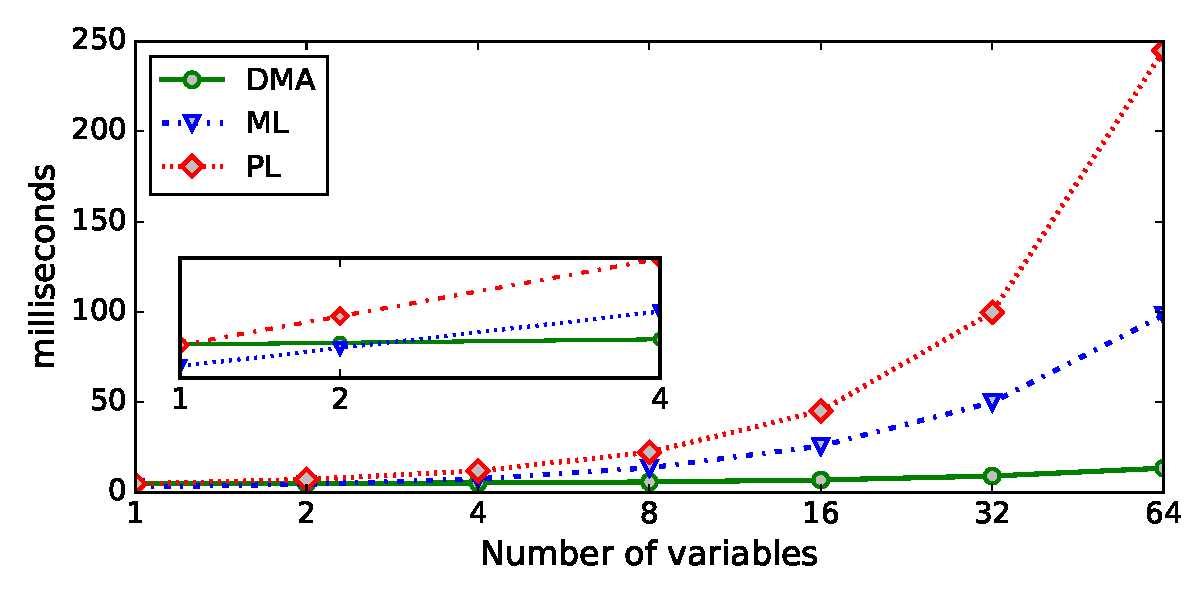
\includegraphics[width=\columnwidth]{figures/iposCommitSize}
%	\caption{Commit size delay for three memory access methods.}
%	\label{fig:virtOperationalBuf}
%\end{figure}


\begin{figure}[t]
	\centering
	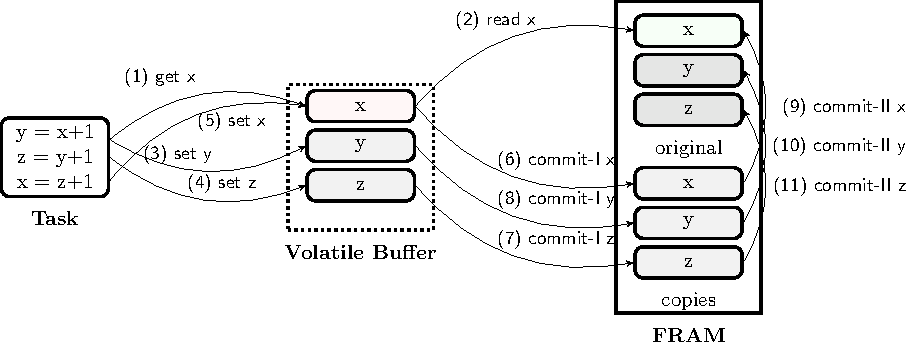
\includegraphics[width=\columnwidth]{figures/sram-buffer}
	\caption{The interaction between the task, volatile buffer and the non-volatile memory (FRAM). Initially, the persistent variable \texttt{x} is not in the volatile buffer but \texttt{y} and \texttt{z} are. }
	\label{fig:volatile-buffer}
\end{figure}


\paragraph{Problem 1---Runtime Access Overhead:} The persistent variables read and/or modified by a task might not be known in advance due to the dynamic program flow. Therefore, the volatile buffer should keep track of the persistent variables at runtime, as presented in Fig.\,\ref{fig:volatile-buffer}. When a persistent variable is read or written---refer steps 1 and 3--5 in this figure, first the volatile copy of the corresponding variable is \emph{searched} in this buffer. If it is found, the read or write operation is performed on the volatile copy. Otherwise, the persistent variable is read from the non-volatile memory and inserted in this buffer for future operations---refer step 2 in Fig.\,\ref{fig:volatile-buffer}. Unfortunately, we observed that \emph{search--bring} operations at each access to the persistent variables introduce considerable overhead and might kill the benefit of task coalescing as we present in Section \ref{sec:task_coalescing}.\todo{How to show it experimentally?}{Maybe we can show one of the results of Amjad?} %refer to Figure~\ref{fig:virtOperationalBuf} for experimental evaluation.

\begin{figure}[t]
	\centering
	\subfloat[Time needed to transfer a block of data]{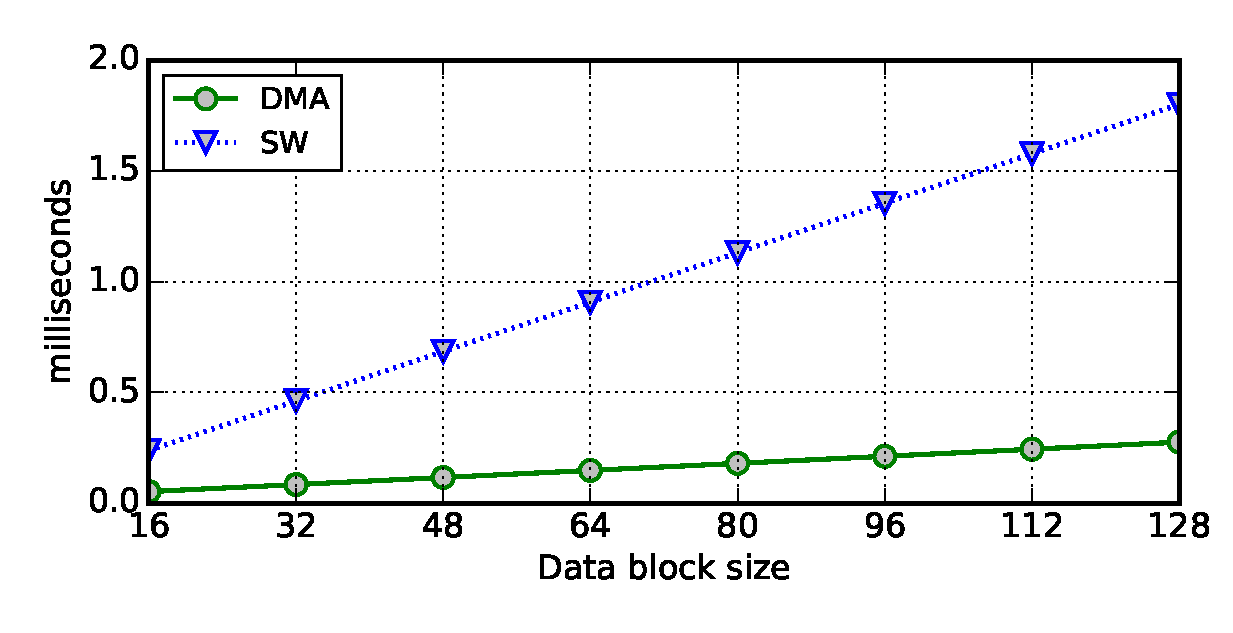
\includegraphics[width=0.49\columnwidth]{figures/dmaSize_time.eps} }
	\subfloat[Energy needed to transfer a block of data]{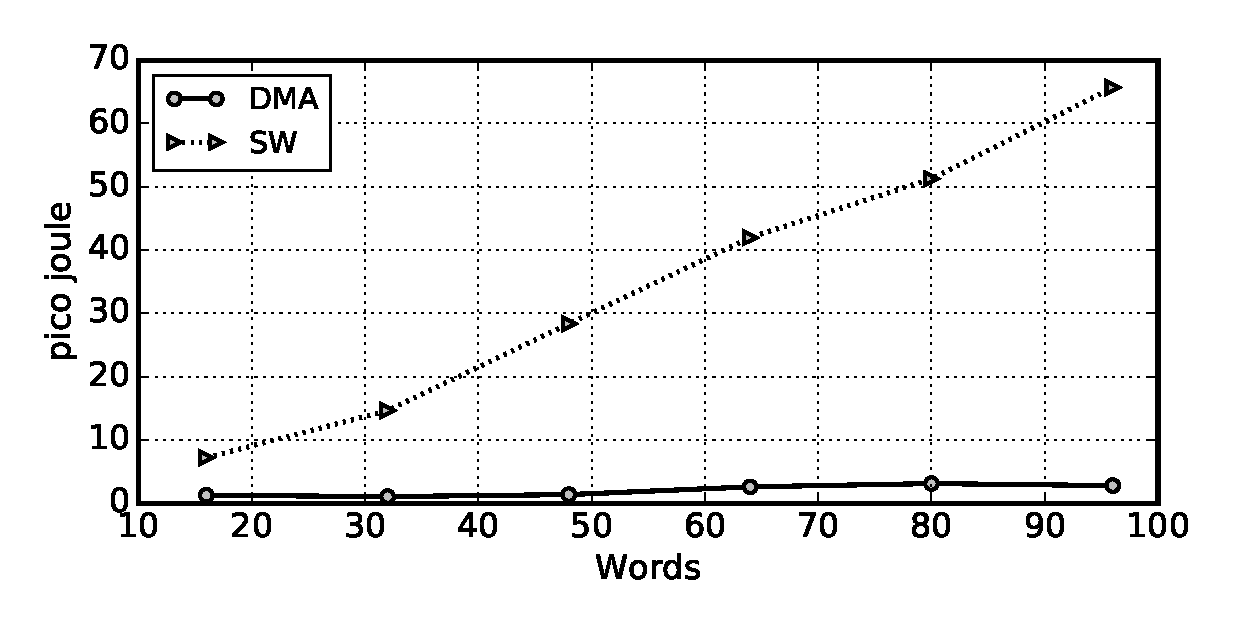
\includegraphics[width=0.49\columnwidth]{figures/energyConsumptionDMA_SW.eps}}
	\caption{Time and energy consumption of moving a block of data from SRAM to FRAM: CPU intervention versus Direct Memory Access (DMA).\todo{Explain HW/SW setup; make fonts larger, unify legends and axes}{Amjad}}
	\label{fig:dmaTimeEnergy}
\end{figure}

\paragraph{Problem 2---Two Phase Commit Overhead:} For the consistency of the non-volatile memory, the volatile buffer should be committed at the end of each task by means of a \emph{two-phase commit} approach---refer Fig.\,\ref{fig:volatile-buffer} steps 6--8 for the first phase and 9--11 for the second step of the commit operation. However, two-phase commit is also expensive since the committed variables are not \emph{contiguous}---leading the fact that copying or moving of data between/within volatile and non-volatile memory should be always performed selectively with CPU intervention. Non-selective block memory copy operations using Direct Memory Access (DMA) that eliminates CPU intervention are considerably more efficient, refer to Fig.~\ref{fig:dmaTimeEnergy} for a comparison, but infeasible in this case.  

\paragraph{Problem 3---Main Memory Constraints:} Persistent variables can be allocated \emph{contiguously} in non-volatile memory with compiler support. In order to eliminate run-time buffer \emph{search} overhead (by not relying on specialized hardware such as e.g. in~\cite{hicks_isca_2017}), \emph{all} persistent variables can be brought from non-volatile memory to the volatile buffer at system start-up---very efficiently and faster thanks to DMA for \emph{block} memory-memory copy/move operations. Two-phase commit is also very efficient in this case since DMA can be utilized to move volatile buffer as a block to the corresponding non-volatile locations. However, bringing all persistent variables from non-volatile memory to the volatile buffer suffers from the \emph{memory fit problem}: the volatile memory is a scarce resource and may not be large enough to hold all persistent variables.

\subsection{Software-based Paging Mechanism}
Considering these facts, \sys implements a \emph{paging-based} virtual memory in software that (i) partitions contiguously allocated persistent variables into pages; (ii) implements the volatile \emph{page buffer} that holds a single page---solves the aforementioned memory-fit problem; (iii) swaps the page in volatile memory with a new page in non-volatile memory efficiently by utilizing DMA-based memory block-copy operations; (iv) buffers the swapped volatile page until commit to enable task coalescing we describe in Section \ref{sec:task_coalescing}; (v) implements two-phase commit of the modified pages to preserve the consistency of non-volatile memory; (vi) and performs two-phase commit operations using DMA for the sake of efficiency. We explain the details of \sys paging mechanism in the following subsections.

\subsubsection{Address Translation and Variable Access}

Our virtual memory system provides an interface to the applications which is composed of two C macros: \texttt{RVAR(var)} and \texttt{WVAR(var,val)} that accept the name of the persistent variable \texttt{var} as an input argument. These macros obtain the \emph{physical address} of the corresponding persistent variable in non-volatile memory and translates it into the \emph{virtual address} in page buffer \texttt{pageBuf} in volatile memory, which is composed of a \emph{page tag} and \emph{offset}. For the sake of simplicity and efficiency, we implemented this translation in a trivial way: the first byte of the physical address is considered to be the page tag and the rest is the offset within the corresponding page. 

\begin{algorithm}[t]
	\caption{\texttt{RVAR(var)} pseudo-code}
	\label{algo:rwar}
	\scriptsize
	%\small
	\begin{algorithmic}[1]
		\State $\texttt{tag}\leftarrow \texttt{getTag(var)}$ 
		\If { \texttt{tag} != \texttt{CrntPagTag} }	\Comment{Check if the page is in page buffer}
		\State	\texttt{PageFault(tag)} \Comment{Page is not in the page buffer, bring it}
		\EndIf
				\State $\texttt{offset}\leftarrow \texttt{getOffset(var)}$ 		
		\State \texttt{return pageBuf[offset]}  \Comment{Return directly from page buffer}
	\end{algorithmic}
\end{algorithm}

After address translation and obtaining the virtual address, it is required to check if the corresponding page is already in volatile page buffer. To this end, our system maintains a \texttt{CrntPagTag} variable that holds the tag of the page currently in the page buffer. If the tag of the virtual address and \texttt{CrntPagTag} are equal, this indicates that page buffer holds the required page and the offset of the virtual address can be used to read from/write to the location in the volatile page buffer immediately. If the required page is not in the page buffer, a \emph{page fault} routine is executed as we discuss in the next subsection. Observe that the computational complexity of the whole steps pertaining to address translation and variable access is $\mathcal{O}(1)$---introducing minimal overhead to the system to boost up benefits of volatile-only memory interfacing. The pseudo-code of \texttt{RVAR}, which is quite similar to that of \texttt{WVAR}, is presented in Algorithm~\ref{algo:rwar}.

\subsubsection{Page Faults and Page Swapping}

\begin{algorithm}[t]
	\caption{\texttt{PageFault(tag)} pseudo-code}
	\label{algo:pagefault}
	\scriptsize
	%\small
	\begin{algorithmic}[1]
		\If {\texttt{isDirty(CrntPagTag)} }	\Comment{Check if the active page is modified}
		\State \texttt{pageCommit(pagesTemp)} \Comment{Phase-I commit the active page}
		\EndIf
		\If {\texttt{isDirty(tag)}} \Comment{Check if the requested page has been modified}
		\State {\texttt{getPage(tag,pagesTemp)}=false} \Comment{Get page from temporary buffer}
		\Else
		\State \texttt{getPage(tag,pagesOrg)}==false \Comment{Get page from original location}
		\EndIf 
		\State \texttt{CrntPagTag} = \texttt{tag} \Comment{Update tag}
	\end{algorithmic}
\end{algorithm}

If the page tag of the variable \texttt{var} and \texttt{CrntPagTag} are not equal (e.g. Lines 2--3 of Algorithm\,\ref{algo:rwar}), the active page, i.e. the contents of the page buffer \texttt{pageBuf}, should be swapped with the page whose tag is equal to the \texttt{var}'s tag. The pseudo-code of the Algorithm \texttt{PageFault} that handles this operation is presented in Algorithm\,\ref{algo:pagefault}. This algorithm handles two fundamental cases:

\paragraph{Modified Active Page:} If the task performed at least \texttt{WVAR} operation, then the page buffer \texttt{pageBuf} that holds the current active page is modified (Line 1 of Alg.\,\ref{algo:pagefault}). In order to keep the modified values of the variables, the active page is committed to an intermediate page buffer in non-volatile memory, namely to \texttt{pagesTemp}. This operation can be considered as first phase of the commit operation, as we present in the next subsection. If the active page is not modified, there is no need to commit it to the temporary page buffer.

\paragraph{Modified Requested Page:} After committing the active page to its temporary location, Algorithm\,\ref{algo:pagefault} checks if the requested page is modified previously by the same task (Line 3). If this is the case, the requested page should be be brought from \texttt{pagesTemp} rather than its original location in non-volatile memory (Line 4), so that the task accesses the modified values of the persistent variables. Otherwise, the requested page is brought from its original location, i.e. \texttt{pagesOrg} (Line 6). After the swapping operation, the \texttt{CrntPagTag} is set to the tag of the requested page (Line 7). It should be noted that DMA is used to memory block copy operations, introducing minimal overhead during page swapping. 

\subsubsection{Pages Final Committing}

After a task finishes its execution, all pages committed to \texttt{pagesTemp} should be committed to their original locations in \texttt{pagesOrg}. This is the second phase of the \emph{two-phase commit} operation. As mentioned previously, memory block copy operations for the second phase commit is also utilized by DMA.

\subsection{Non-Volatile Memory Consistency Issues}  
During the execution of any task, modifications to the persistent variables will not be reflected to the original locations in the non-volatile memory, since the task interfaces with only the volatile page buffer \texttt{pageBuf} and the modifications are temporarily stored in the non-volatile \texttt{pagesTemp} buffer. The changes stored in the \texttt{pagesTmp} is committed to the original locations in \texttt{pagesOrg} after the task is finished its execution. Therefore, any power interruptions within the execution will not lead to inconsistencies in the \texttt{pagesOrg} when the task is re-executed after a power boot. As a consequence, the proposed paging mechanism keeps the consistency of the non-volatile memory thanks to the two-phase commit operation for the modified pages. 
\todo{Benefits of the paging to the task coalescing should be mentioned in the next section}{Amjad/Przemek/Sinan}